\documentclass[12pt,a4paper]{article}

\usepackage[french]{babel}
\usepackage[utf8]{inputenc}
\usepackage[T1]{fontenc}
\usepackage{fouriernc}
\usepackage{geometry}
\usepackage{array}
\usepackage{booktabs}
\usepackage{tabularx}
\usepackage[table]{xcolor}
\usepackage{amsmath}
\usepackage{fancyhdr}
\usepackage{tikz}
\usepackage{pgfplots}
\usepackage[most]{tcolorbox}
\usepackage{enumitem}
\pgfplotsset{compat=1.18}

\geometry{top=2.2cm, bottom=2cm, left=2cm, right=2cm, headheight=15pt}

%------------------------------------------------------------
% Couleurs (identiques au modèle activite_propagation_son_TRPM)
%------------------------------------------------------------
\definecolor{bluedark}{RGB}{50, 100, 160}
\definecolor{bluelight}{RGB}{210, 228, 248}
\definecolor{bluemid}{RGB}{170, 200, 235}
\definecolor{grisfond}{RGB}{245, 245, 245}

%------------------------------------------------------------
% En-tête / pied de page
%------------------------------------------------------------
\pagestyle{fancy}
\fancyhf{}
\lhead{\small Physique-Chimie -- Première Bac Pro Microtechniques}
\rhead{\small Les solutions aqueuses}
\cfoot{\thepage}
\renewcommand{\headrulewidth}{0.5pt}

%------------------------------------------------------------
% Boîtes tcolorbox
%------------------------------------------------------------
\tcbset{
  stylepartie/.style={
    colback=bluedark,
    colframe=bluedark,
    coltext=white,
    fonttitle=\bfseries,
    boxrule=0pt,
    arc=3pt,
    left=6pt, right=6pt, top=4pt, bottom=4pt,
    before skip=10pt, after skip=6pt,
  },
  styledoc/.style={
    colback=bluelight,
    colframe=bluemid,
    boxrule=0.8pt,
    arc=3pt,
    left=8pt, right=8pt, top=5pt, bottom=5pt,
    before skip=6pt, after skip=4pt,
    fonttitle=\bfseries\small,
    attach boxed title to top left={yshift=-2mm, xshift=4mm},
    boxed title style={colback=bluemid, colframe=bluemid, arc=2pt},
  },
  styleinfo/.style={
    colback=grisfond,
    colframe=bluemid,
    boxrule=0.8pt,
    arc=3pt,
    left=8pt, right=8pt, top=5pt, bottom=5pt,
    before skip=6pt, after skip=6pt,
  },
}

%------------------------------------------------------------
% Commandes utiles
%------------------------------------------------------------
\newcommand{\cadrecalcul}[1][4cm]{%
  \vspace{5mm}%
  \begin{tcolorbox}[
    colback=white,
    colframe=bluemid,
    boxrule=0.8pt,
    arc=4pt,
    left=4pt, right=4pt,
    top=0pt, bottom=0pt,
    height=#1,
    after skip=2mm,
  ]
  \end{tcolorbox}%
}

\newcommand{\reponse}[1]{%
  \vspace{5mm}%
  \foreach \i in {1,...,#1}{%
    \par\noindent\makebox[\linewidth]{\dotfill}\vspace{2mm}%
  }%
}

\newcounter{numquestion}
\newcommand{\question}[1]{%
  \stepcounter{numquestion}%
  \vspace{6pt}%
  \noindent{\color{bluedark}$\blacktriangleright$~\textbf{Question~\thenumquestion.}}~#1%
  \vspace{2pt}%
}

%------------------------------------------------------------
\begin{document}
%------------------------------------------------------------

%============================================================
% TITRE
%============================================================
\begin{tcolorbox}[
  colback=white, colframe=bluedark, boxrule=1.5pt, arc=4pt,
  before skip=0pt, after skip=8pt,
  left=10pt, right=10pt, top=8pt, bottom=8pt,
]
  \begin{center}
    {\color{bluedark}\Large\bfseries Dissolution et Dilution}\\[4pt]
    {\large Activité documentaire}\\[6pt]
    \hrule height 0.4pt \vspace{6pt}
    \textbf{Durée :} 1\,h\,00 \hfill \textbf{Niveau :} Première Bac Pro
  \end{center}
\end{tcolorbox}

\vspace{2pt}
\noindent\rule{\linewidth}{0.5pt}
\vspace{4pt}

\noindent\textbf{Nom :} \dotfill \hspace{1cm} \textbf{Prénom :} \dotfill \hspace{1cm} \textbf{Classe :} \dotfill

\vspace{2pt}
\noindent\rule{\linewidth}{0.5pt}
\vspace{6pt}

%------------------------------------------------------------
% Compétences
%------------------------------------------------------------
\begin{tcolorbox}[styleinfo]
  \textbf{\color{bluedark}Compétences travaillées (référentiel)}
  \begin{itemize}[noitemsep, leftmargin=1.2em]
    \item Extraire des informations de documents scientifiques et les exploiter.
    \item Distinguer dissolution et dilution ; identifier soluté et solvant.
    \item Utiliser les relations $C_m = m/V$, $n = m/M$ et $C_1 V_1 = C_2 V_2$.
    \item Calculer une concentration massique ou molaire à partir de données expérimentales.
  \end{itemize}
\end{tcolorbox}

%------------------------------------------------------------
% Contexte
%------------------------------------------------------------
\begin{tcolorbox}[styleinfo]
  \textbf{\color{bluedark}Contexte}\\[4pt]
  Dans un atelier de microtechniques, les pièces mécaniques (engrenages, axes, micro-composants)
  doivent être \textbf{nettoyées}, \textbf{dégraissées} et parfois \textbf{décapées} avant
  assemblage ou contrôle de conformité. Ces opérations font appel à des \textbf{solutions
  aqueuses} préparées avec soin, dont la concentration doit être parfaitement maîtrisée.
  Dans cette activité, vous allez comprendre comment préparer ces solutions par
  \textbf{dissolution} ou par \textbf{dilution}.
\end{tcolorbox}

\vspace{4pt}

%============================================================
% PARTIE A
%============================================================
\begin{tcolorbox}[stylepartie]
  Partie A -- La dissolution : préparer une solution à partir d'un solide \hfill {\normalfont\small (20 min)}
\end{tcolorbox}

%------------------------------------------------------------
% Document 1
%------------------------------------------------------------
\begin{tcolorbox}[styledoc, title={Document 1 -- Préparation d'une solution saline en atelier}]
  Dans certains ateliers de microtechniques, on utilise une \textbf{solution aqueuse de
  chlorure de sodium} (NaCl) comme bain de rinçage non corrosif. Cette solution est préparée
  par \textbf{dissolution} d'un soluté solide dans de l'eau distillée.

  \medskip

  \textbf{Protocole :} un technicien pèse $m = 4{,}5$~g de chlorure de sodium (NaCl),
  l'introduit dans une fiole jaugée de $V = 500$~mL, puis complète avec de l'eau distillée
  jusqu'au trait de jauge.

  \medskip

  \textbf{Définitions :}
  \begin{itemize}[noitemsep, leftmargin=1.5em]
    \item Le \textbf{soluté} est l'espèce dissoute (solide ou liquide).
    \item Le \textbf{solvant} est le liquide dans lequel on dissout (ici l'eau).
    \item La \textbf{solution} est le mélange homogène obtenu.
  \end{itemize}

  \medskip

  La \textbf{concentration massique} $C_m$ quantifie la masse de soluté par litre de
  solution :
  \[
    C_m = \dfrac{m_{\text{soluté}}}{V_{\text{solution}}}
    \qquad
    \bigl(C_m \text{ en g/L},\; m \text{ en g},\; V \text{ en L}\bigr)
  \]

  \medskip
  \textit{Données :} Masses molaires atomiques -- Na : 23~g/mol ; Cl : 35,5~g/mol.
\end{tcolorbox}

\newpage

\question{Identifier dans le texte le \textbf{soluté} et le \textbf{solvant} de la solution préparée.}
\reponse{2}

\question{Calculer la masse molaire $M(\text{NaCl})$ du chlorure de sodium (en g/mol).}
\cadrecalcul[1.8cm]

\question{Calculer la concentration massique $C_m$ (en g/L) de la solution. \textit{Attention à
l'unité du volume.}}
\cadrecalcul[2.3cm]

%============================================================
% PARTIE B
%============================================================
\begin{tcolorbox}[stylepartie]
  Partie B -- La dilution : préparer une solution à partir d'une solution concentrée \hfill {\normalfont\small (20 min)}
\end{tcolorbox}

%------------------------------------------------------------
% Document 2
%------------------------------------------------------------
\begin{tcolorbox}[styledoc, title={Document 2 -- Dilution d'un dégraissant industriel}]

  Un dégraissant industriel est commercialisé sous forme de \textbf{solution mère} concentrée
  à $C_1 = 80$~g/L. Pour des raisons de sécurité et d'efficacité, il doit être \textbf{dilué}
  avant emploi dans le bain ultrasonique de l'atelier.

  \medskip

  Le technicien doit préparer $V_2 = 2{,}0$~L de \textbf{solution fille} de concentration
  $C_2 = 10$~g/L en prélevant un volume $V_1$ de solution mère et en complétant à 2,0~L
  avec de l'eau distillée.

  \medskip

  \textbf{Propriété fondamentale de la dilution :} la quantité de soluté est
  \textbf{conservée} entre la solution mère et la solution fille :
  \[
    \boxed{C_1 \times V_1 = C_2 \times V_2}
  \]

  Le \textbf{facteur de dilution} est : $f = \dfrac{C_1}{C_2} = \dfrac{V_2}{V_1}$

  \vspace{4pt}

  \begin{center}
    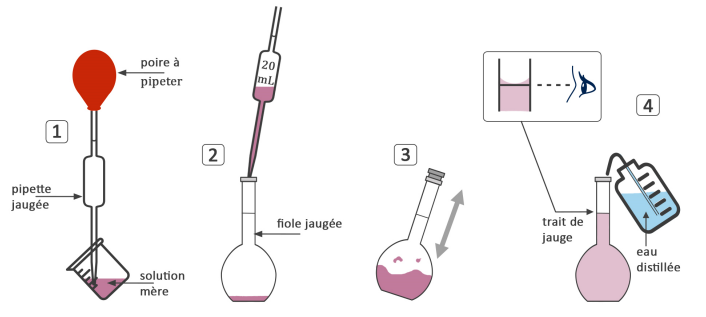
\includegraphics[width=0.7\linewidth]{images/dilution2.png}
  \end{center}

\end{tcolorbox}

\newpage

\question{Expliquer, en une phrase, ce qu'est une \textbf{dilution} et ce qui est conservé lors de cette opération.}
\reponse{2}

\question{Calculer le \textbf{facteur de dilution} $f$ entre la solution mère et la solution fille.}
\cadrecalcul[1.8cm]

\question{En utilisant la relation $C_1 V_1 = C_2 V_2$, calculer le volume $V_1$ (en mL) de solution mère à prélever.}
\cadrecalcul[2.5cm]

%------------------------------------------------------------
% Document 3 -- Verrerie et protocole de dilution
%------------------------------------------------------------
\begin{tcolorbox}[styledoc, title={Document 3 -- La verrerie utilisée en chimie et protocole de dilution}]

  \begin{minipage}[t]{0.62\linewidth}
    \textbf{Les principaux instruments de mesure de volume :}

    \vspace{4pt}
    \begin{itemize}[noitemsep, leftmargin=1.4em]
      \item \textbf{Éprouvette graduée} : mesure approchée d'un volume de liquide.
      \item \textbf{Pipette graduée} : permet de prélever un volume quelconque avec précision.
      \item \textbf{Fiole jaugée} : contient un volume \textit{exact} (trait de jauge gravé) ; sert à préparer une solution de volume précis.
      \item \textbf{Pissette d'eau distillée} : utilisée pour compléter au trait de jauge sans dépasser.
    \end{itemize}

    \vspace{8pt}
    \textbf{Protocole de dilution en 4 étapes :}

    \vspace{4pt}
    \begin{enumerate}[noitemsep, leftmargin=1.6em, label=\textbf{\arabic*.}]
      \item Prélever le volume $V_1$ de solution mère à l'aide d'une \textbf{pipette graduée}.
      \item Verser dans une \textbf{fiole jaugée} de volume $V_2$.
      \item Compléter \textit{progressivement} avec de l'eau distillée jusqu'au \textbf{trait de jauge}.
      \item Boucher et \textbf{agiter} pour homogénéiser la solution.
    \end{enumerate}
  \end{minipage}
  \hfill
  \begin{minipage}[t]{0.34\linewidth}
    \vspace{0pt}
    \begin{center}
      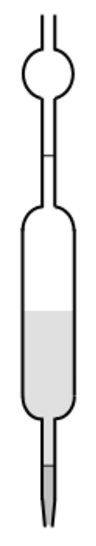
\includegraphics[height=4.5cm]{images/pipette.pdf}
      \hspace{1.5cm}
      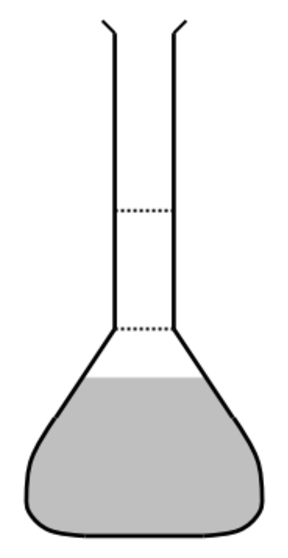
\includegraphics[height=4.5cm]{images/fiole.pdf}

      \vspace{2mm}
      {\scriptsize\hspace{0.5cm}Pipette graduée\hspace{2.8cm}Fiole jaugée}
    \end{center}
  \end{minipage}

\end{tcolorbox}

\newpage

\question{En vous aidant du document~3, nommer le matériel que le technicien doit utiliser pour prélever $V_1$ avec précision, puis pour préparer la solution fille. Justifier.}
\reponse{2}


%============================================================
% PARTIE C
%============================================================
\begin{tcolorbox}[stylepartie]
  Partie C -- Concentration molaire et bilan de synthèse \hfill {\normalfont\small (20 min)}
\end{tcolorbox}

%------------------------------------------------------------
% Document 4
%------------------------------------------------------------
\begin{tcolorbox}[styledoc, title={Document 4 -- Fiche de données de sécurité d'un produit de décapage}]

  Pour décaper les pièces en aluminium avant soudage, l'atelier utilise une solution d'acide
  citrique. Voici un extrait de sa fiche de données de sécurité (FDS) :

  \vspace{6pt}
  \begin{center}
  \renewcommand{\arraystretch}{1.4}
  \begin{tabular}{|p{0.44\linewidth}|p{0.44\linewidth}|}
    \hline
    \rowcolor{bluemid}
    \textbf{Paramètre} & \textbf{Valeur} \\
    \hline
    Nom du produit & Acide citrique \\
    \hline
    Formule chimique & $\mathrm{C_6H_8O_7}$ \\
    \hline
    Masse molaire & $M = 192$~g/mol \\
    \hline
    Concentration massique du bain & $C_m = 96$~g/L \\
    \hline
    Volume du bain ultrasonique & $V = 5{,}0$~L \\
    \hline
    Seuil de remplacement du bain & $C < 0{,}25$~mol/L \\
    \hline
  \end{tabular}
  \end{center}

  \vspace{6pt}

  La \textbf{concentration molaire} $C$ (en mol/L) est liée à la concentration massique
  $C_m$ (en g/L) par :
  \[
    C = \dfrac{C_m}{M}
  \]

  La \textbf{quantité de matière} de soluté dans le bain est :
  \[
    n = C \times V \qquad \bigl(n \text{ en mol},\; C \text{ en mol/L},\; V \text{ en L}\bigr)
  \]

\end{tcolorbox}

\question{Calculer la \textbf{concentration molaire} $C$ (en mol/L) de la solution d'acide citrique du bain.}
\cadrecalcul[2.3cm]

\question{Calculer la \textbf{quantité de matière} $n$ d'acide citrique contenue dans le bain de 5,0~L.}
\cadrecalcul[2.3cm]

\question{\textbf{Décision :} Le bain doit être renouvelé si $C < 0{,}25$~mol/L.
À partir du résultat de la question~8, \textbf{conclure} si le bain est encore utilisable.}
\reponse{2}

%------------------------------------------------------------
% Document 4
%------------------------------------------------------------
\begin{tcolorbox}[styledoc, title={Document 5 -- Synthèse : dissolution ou dilution ?}]

  \begin{center}
  \renewcommand{\arraystretch}{1.5}
  \begin{tabular}{|p{0.21\linewidth}|p{0.34\linewidth}|p{0.34\linewidth}|}
    \hline
    \rowcolor{bluemid}
    & \textbf{Dissolution} & \textbf{Dilution} \\
    \hline
    \textbf{Point de départ} & Soluté \textbf{solide} + solvant & Solution \textbf{concentrée} (mère) \\
    \hline
    \textbf{Ce qu'on ajoute} & Solvant (eau distillée) & Solvant (eau distillée) \\
    \hline
    \textbf{Ce qui est conservé} & La masse du soluté & La quantité de soluté ($C_1 V_1 = C_2 V_2$) \\
    \hline
    \textbf{Matériel clé} & Balance + fiole jaugée & Pipette + fiole jaugée \\
    \hline
    \textbf{Exemple dans l'atelier} & Solution saline (NaCl) & Bain dégraissant dilué \\
    \hline
  \end{tabular}
  \end{center}

\end{tcolorbox}

\question{\textbf{Synthèse :} En vous appuyant sur le document~5, expliquer en vos propres mots
la \textbf{différence fondamentale} entre une dissolution et une dilution. Donner un exemple
de chaque opération rencontré dans cette activité.}
\reponse{4}

\vspace{8pt}
\begin{center}
  \color{bluedark}\rule{0.5\linewidth}{0.6pt}
\end{center}

\end{document}
